\documentclass[a4paper]{article}

% Paketimporte
\usepackage[ngerman]{babel} % Neue Deutsche Rechtschreibung
\usepackage[utf8]{inputenc} % UTF-8 für plattformunabhängige Codierung mit Umlauten
\DeclareUnicodeCharacter{00A0}{ } % Für no-break-spaces
\usepackage{eurosym} % €-Symbol
\usepackage{titlesec} % Textüberschriften anpassen
\usepackage[pdftex]{graphicx} % Für Grafiken
\usepackage{float} 
\usepackage{url} % Für korrekte URL-Formatierung
\usepackage{wrapfig} % Für Abbildungen mit textumlauf
\usepackage{csquotes} % Für Zitate
\usepackage{glossaries} % Für Glossar
\usepackage[markup=nocolor,deletedmarkup=xout]{changes} % Für Änderungen
\usepackage[section]{placeins} % Für floar barrier

% \titleformat{⟨Überschriftenklasse⟩}[Absatzformatierung⟩]{⟨Textformatierung⟩} {⟨Nummerierung⟩}{⟨Abstand zwischen Nummerierung und Überschriftentext⟩}{⟨Code vor der Überschrift⟩}[⟨Code nach der Überschrift⟩]

\titleformat{\chapter}[hang]{\large\bfseries}{\thechapter\quad}{0pt}{}
\titleformat{\section}[hang]{\large\bfseries}{\thesection\quad}{0pt}{}
\titleformat{\subsection}[hang]{\large\bfseries}{\thesubsection\quad}{0pt}{}
\titleformat{\subsubsection}[hang]{\large\bfseries}{\thesubsubsection\quad}{0pt}{}
\titleformat{\paragraph}[hang]{\large\bfseries}{\theparagraph\quad}{0pt}{}

% \titlespacing{⟨Überschriftenklasse⟩}{⟨Linker Einzug⟩}{⟨Platz oberhalb⟩}{⟨Platz unterhalb⟩}[⟨rechter Einzug⟩]

\titlespacing{\chapter}{0pt}{-3em}{6pt}
\titlespacing{\section}{0pt}{6pt}{6pt}
\titlespacing{\subsection}{0pt}{6pt}{6pt}
\titlespacing{\subsubsection}{0pt}{6pt}{6pt}
\titlespacing{\paragraph}{0pt}{6pt}{6pt}

%Toleranzen für Mikrotypographie
\pretolerance=150
\setlength{\emergencystretch}{10em}

% Metadaten
\title{Anforderungsspezifikation zum Projekt \linebreak \enquote{DSCMS4}}
\author{HOMEINFO - Digitale Informationssysteme GmbH}
\date{\today}

% Inhaltsverzeichnis-Konfiguration
\setcounter{tocdepth}{5}
\setcounter{secnumdepth}{5}

% Glossar
\makeglossaries
	
\begin{document}	
	% Titelblatt
	\maketitle
	\pagebreak
	
	% Inhaltsverzeichnis
	\tableofcontents
	\pagebreak
	
	\section*{Vorwort}
	Diese Spezifikation stellt fest, was entwickelt werden soll. Sie enthält dazu die Anforderungen des Kunden an die Anwendung.
	Vermerke und ausstehende Aktionen sind \emph{kursiv} gedruckt.
	\section*{Änderungsliste}
	\begin{itemize}
		\item 09.03.2017
		\begin{itemize}
			\item Erstellung des Dokuments.
		\end{itemize}
	\end{itemize}
	
	\pagebreak
	\section{Mission des Projekts}
	Ziel ist es, ein Content Management System (\enquote{CMS}) Zur Verfügung zu stellen, in welchem die Kunden von HOMEINFO \emph{Mieteinheiten}, \emph{Standorte} und \emph{Gruppen} pflegen können.
	Die bisherigen Funktionen des \enquote{Digital Signage Content Management Systems, Version 3} (\emph{DSCMS3}) sollen zum Teil vom neuen System übernommen und optimiert werden um das DSCMS3 ablösen.
	Dies beinhaltet das Verwalten von sog. \enquote{Charts} und \emph{Konfigurationen}.
	Diese Elemente sollen ebenfalls mit den Elementen der Unternehmensstruktur assoziiert werden können.
	\subsection{Abbildung der Unternehmensstrukturen der Kunden}
	Das DSCMS4 soll es den Kunden ermöglichen, ihre internen Strukturen abzubilden. Dies soll durch die Definition von \emph{Mieteinheiten}, \emph{Standorten} sowie \emph{Gruppen} erreicht werden.
	\subsubsection{Mieteinheiten}
	Mieteinheiten sind optional von Kunden, insbesondere solchen aus der Wohnungswirtschaft, nutzbar und sollen durch HOMEINFO für den Kunden aus deren Datenbeständen vorkonfiguriert werden können. Jede Mieteinheit ist genau einem Standort zugeordnet und besteht aus einer \emph{ID} sowie einer \emph{optionalen} Beschreibung. Mieteinheiten sollen die Schnittstelle zu den in \emph{ComCat} verwendeten Mieteraccounts bilden.
	\subsubsection{Standorte}
	Standorte stellen Tupel aus \emph{Name}, \emph{Beschreibung} und \emph{Adresse} dar. Sie sollen dazu dienen Standorte für Digital Signage \emph{Terminals} abzubilden sowie Kunden der Wohnungswirschaft die Möglichkeit zu bieten, Verwaltungseinheiten (\enquote{VE}) abzubilden.
	\subsubsection{Gruppen}
	Gruppen sollen dem Kunden zur Abbildung seiner Unternehmensstruktur oder auch allgemein zur Organisation der Verwaltungseinheiten und Standorte dienen.
	Gruppen können Mieteinheiten, Standorte oder andere Gruppen als Mitglieder haben, wobei Zyklen zu vermeiden sind.
	Gruppen sollen einen Namen und eine optionale Beschreibung aufweisen.
	\subsection{Erstellung und Verwaltung von Inhalten}
	Inhalte bezeichnen im Sinne dieses Dokuments Informationen, welche der Kunde auf seinen Digital Signage Systemen anzeigen lassen möchte sowie solche Informationen, die an die Mieter-Apps des \emph{ComCat} Systems übertragen werden sollen.
	\subsubsection{Verfügbare Inhalte}
	Im DSCMS4 sollen folgende Typen von Inhalten Zur Verfügung gestellt werden.
	\paragraph{Charts}
	Bei den sogenannten \enquote{Charts} handelt es sich um Datenstrukturen, welche eine geschlossene Informationseinheit in den Digital Signage Anwendungen repräsentieren.
	Aktuell sind folgende Charts vorgesehen:
	\subparagraph{Generischer Chart}
	Bei dem generischen Chart handelt es sich um eine abstrakte Datenstruktur, welche die Basis für alle folgenden Chart-Typen, soweit nicht anders beschrieben, darstellt.
	Der generische Chart hat folgende Attribute:
	\begin{itemize}
	\item Kunde
	\item Autor
	\item Titel
	\item Untertitel
	\item Anzeigedauer
	\item Erstellungsdatum
	\item Index
	\item Zeitplan
	\end{itemize}
	\subparagraph{HTML Chart}
	Bei dem HTML-Chart handelt es sich um eine Erweiterung des Basis Charts, welche einen HTML Text und beliebig viele Bilder enthält.
	\begin{itemize}
	\item Text
	\item Bilder
		\begin{itemize}
		\item Bild1
		\item Bild2
		\item ...
		\end{itemize}
	\end{itemize}
	Der HTML-Chart stellt eine Synthese der beiden ehemaligen Chart Typen \emph{BildTextChart} und \emph{PinChart} dar.
	\subparagraph{Text Chart}
	Der Text-Chart stellt eine einfachere Variante des HTML Charts dar und verfügt gegenüber dem Basis Chart lediglich über einen zusätzlichen Text.
	\begin{itemize}
	\item Text
	\end{itemize}
	\subparagraph{Video Chart}
	Der Video-Chart erweitert den Basis Chart lediglich um ein Video.
	\begin{itemize}
	\item Video
	\end{itemize}
	\paragraph{Zusätzliche Charts}
	Zusätzliche Charts leiten sich, sofern nicht anders beschreiben. ebenfalls vom o.g. generischen Chart ab, sollen jedoch nur verwendet werden können, sofern der entsprechende Dienst von Kunden bei HOMEINFO gebucht wurde.
	\subparagraph{Nachrichten}
	Der Nachrichten-Chart zeigt internationale Nachrichten des Dienstes \emph{Adversign} an. Er erweitert den generischen Chart um keine zusätzlichen Attribute.
	\subparagraph{Lokale Nachrichten}
	Der Chart für lokale Nachrichten soll Nachrichten einer entsprechenden Region anzeigen. Die Implementation einer entsprechenden Quelle steht noch aus. Der Chart für lokale Nachrichten erweitert den generischen Chart um das Attribut
	\begin{itemize}
	\item Lokalisation
	\end{itemize}
	\subparagraph{Lokale Veranstaltungen}
	Der Chart für lokale Veranstaltungen soll Veranstaltungen in und um den jeweiligen Standort anzeigen. Diese Daten werden einer noch zu entwickelnden Quelle entnommen werden.
	\begin{itemize}
	\item Lokalisation
	\item Zeitspanne (Tage in Zukunft)
	\item Einträge (max.)
	\end{itemize}
	\subparagraph{Zitate}
	Der Zitate-Chart zeigt zufällig ausgewählte Zitate an. Er erweitert den generischen Chart um keine weiteren Attribute.
	\subparagraph{Facebook}
	Der Facebook-Chart zeigt Facebookmeldungen des jeweiligen Kunden an.
	Er erweitert den generischen Chart um folgende Attribute:
	\begin{itemize}
	\item Tage (Anzahl der letzten Tage)
	\item Beiträge (Anzahl der letzten Beiträge)
	\item Facebook ID
	\item Facebook Name
	\end{itemize}
	\subparagraph{Bilderraten}
	Der Bilderraten-Chart zeigt zufällige, verdeckte Bilder, welche im Laufe der Zeit partiell aufgedeckt werden, bis das gesamte Bild zu sehen ist und zeigt am Ende die Bildbeschreibung als Auflösung an.
	Der Bilderraten Chart erweitert den generischen Chart um keine weiteren Attribute.
	\subparagraph{Wetter}
	Der Wetter-Chart zeigt die aktuelle, lokale Wettervorhersage an.
	Er erweitert den generischen Chart um folgendes Attribut:
	\begin{itemize}
	\item Ort
	\end{itemize}
	\subparagraph{ÖPNV Anschlüsse}
	Der ÖPNV-Chart zeigt die nächstgelegenen Haltestellen um Abfahrzeiten für öffentliche Verkehrsmittel.
	Er erweitert den generischen Chart um folgendes Attribut:
	\begin{itemize}
	\item Standort
	\end{itemize}
	\subparagraph{Abfuhrtermine}
	Der Abfuhrtermine-Chart zeigt die nächsten Müllabfuhrtermine für den jeweiligen Standort an.
	Er erweitert den generischen Chart um folgendes Attribut:
	\begin{itemize}
	\item Standort
	\end{itemize}
	\subparagraph{Immobilien}
	Der Immobilien-Chart zeigt die Immobilien des jeweiligen Kunden an.
	Er erweitert den generischen Chart um folgende Attribute:
	\begin{itemize}
	\item QR Code
	\item Bilder Strecken
	\item Stil
	\item Kontaktbild
	\item Übergangseffekt
	\item Kontakt
	\item Ken Burns Effekt
	\item Objektnummer
	\item PLZ Whitelist (Anzuzeigende Postleitzahlen)
	\item PLZ Blacklist (Auszublendende Postleitzahlen)
	\item Mietobjekt
	\item Kaufobjekt
	\item Erbpachtobjekt
	\item Leasingobjekt
	\item Wohnobjekt
	\item Gewerbeobjekt
	\item Anlage
	\item Wohnen auf Zeit
	\end{itemize}
	\subparagraph{Reinigungsplan}
	Der Reinigungsplan-Chart zeigt an, wann welche Reinigungen erfolgt sind (s. Modul \emph{Reinigungsnachweise}).
	Er erweitert den generischen Chart um keine weiteren Attribute.
	\paragraph{Menüs}
	Menüs dienen der Navigation zu Charts auf interaktiven Systemen.
	Menüs stellen eine Baumstruktur dar. Jeder Menübutton ist genau einem oder keinem (\enquote{\emph{root}}) übergeordneten Menübutton zugeordnet.
	Ein Menübutton hat folgende Attribute:
	\begin{itemize}
	\item Name
	\item Bild
	\item Hintergrundfarbe
	\item Textfarbe
	\item Chart
	\item Index
	\end{itemize}
	\paragraph{Ticker}
	Bei dem Ticker handelt es sich um einen Lauftext, welcher entsprechend konfigurierte Inhalte anzeigt.
	Der Ticket hat folgende Attribute:
	\begin{itemize}
	\item Name
	\item Texte
	\item URLs
	\end{itemize}
	\paragraph{Reinigungsnachweis}
	Der Reinigungsnachweis stellt eine Eingabemaske, zur Verfügung, welche per PIN benutzt werden kann, um eine erfolgte Reinigung des entsprechenden Gebäudes einzutragen.
	Der Reinigungsnachweis hat folgendes Attribut:
	\begin{itemize}
	\item Standort
	\end{itemize}
	\paragraph{Kontaktformular}
	Das Kontaktformular erlaubt es an einem interaktiven Digital Signage System dem Vermieter eine Nachricht zukommen zu lassen.
	Das Kontaktformular hat folgenden Attribute:
	\begin{itemize}
	\item Betreff
	\item Nachricht
	\item Kategorie
	\item Schlagworte
	\end{itemize}
	\paragraph{Konfigurationen}
	Konfigurationen sind im Wesentlichen Einstellungen das Design der Digital Signage Anwendung betreffend.
	Es können folgende Parameter konfiguriert werden:
	\begin{itemize}
	\item Schriftart
	\item Schriftgröße
	\item TODO: Vervollständigung durch Raphael!
	\end{itemize}
	\subsubsection{Zuweisung von Inhalten}
	Inhalte können \emph{Mieteinheiten}, \emph{Standorten} und \emph{Gruppen} zugewiesen werden.
	Wird ein Inhalt einer Mieteinheit zugewiesen, so ist der entsprechende Inhalt nur für diese Mieteinheit gültig. Wird ein Inhalt einem Standort zugewiesen, so ist dieser Inhalt für den entsprechenden Standort und alle zugehörigen Mieteinheiten gültig. Wird ein Inhalt einer Gruppe zugewiesen, so ist dieser Inhalt für alle Mitglieder der Gruppe (rekursiv) gültig.
	\subsection{Wünsche und Prioritäten des Kunden}
	\begin{itemize}
		\item Einfache und intuitive Bedienung
		\item Sicherheit und Integrität der erhobenen Daten
		\item Modularität und Erweiterbarkeit
		\item Einhaltung von Standards
	\end{itemize}
		
	\subsection{Domäne}
	Die Domäne beschränkt sich auf Digital Signage und ist spezialisiert auf die Wohnungswirtschaft und die Kommunikation zwischen Vermieter, Mieter und Dienstleister.
	Das System soll jedoch ebenfalls von Kunden, welche nicht aus der Wohnungswirtschaftsbranche stammen genutzt werden können. Daher werden Mieteinheiten als ein optionales Feature implementiert.

	\subsection{Maßnahmen zur Anforderungsanalyse}
	Zur Anforderungsanalyse wurden alleine die \emph{Ideen} und \emph{Vorstellungen} des Geschäftsführers Herrn Gunkel genommen.
	Konkrete Kunden sind nicht vorhanden und Anforderungen potentieller Kunden nicht bekannt.
	Zur Kommunikation dieser Ideen und Vorstellungen wurden \emph{Meetings} mit den Softwareentwicklern \emph{Haupt} und \emph{Neumann} an folgenden Terminen abgehalten:
	\begin{center}
		\begin{tabular}{|p{\dimexpr 0.25\linewidth-2\tabcolsep}|p{\dimexpr 0.75\linewidth-2\tabcolsep}|}
			\hline
			\emph{Datum} & \emph{Thema} \\
			\hline
			Di., 22.11.2016 & Mitteilung und Diskussion der \emph{Ideen} und \emph{Vorstellungen} des Geschäftsführers. \\
			\hline
			Do., 15.12.2016 &Meeting mit den Entwicklern Haupt und Neumann zur Definition der zu übermittelnden Informationen (Titel, Bild, Text...).
       		Diskussion bestehendes CMS weiterentwickeln oder Neuaufbauen
			\\
			\hline
			Di., 15.02.2017 & Meeting mit den Entwicklern Haupt und Neumann zur Analyse der Beziehungen der Entitäten. \\
			\hline
			Mi., 22.02.2017 & Telefonkonferenz mit den Entwicklern Haupt und Neumann zur Analyse der Beziehungen der Entitäten. \\
			\hline
			Mi., 08.03.2017 & Meeting mit den Entwicklern Haupt und Neumann zur Feinabstimmung der Inhalte, Abbildung der Unternehmensstruktur und Zuweisung von Inhalten. \\
			\hline	
		\end{tabular}
	\end{center}
	
	\pagebreak
	\section{Rahmenbedingungen und Umfeld}
	Zur Lösung des Problems soll ein neues Content Management System, das DSCMS4, entwickelt werden, welches auf das HIS-Framework aufbauen soll um die geforderte Modularität und Erweiterbarkeit zu gewährleisten.
	Frontend und Backend sollen über eine JSON-basierte ReST API gekoppelt werden.
	Zur Sicherstellung der Integrität und Sicherheit der erhobenen Daten, sollen sowohl das Frontent, als auch das Backend ausschließlich über HTTPS betrieben werden.
	\subsection{Einschränkungen und Vorgaben}
	Der Entwurf ist gemäß HTTP auf das Client-Server-Modell beschränkt.
	
	\subsection{Anwender}	
	\begin{tabular}{|p{\dimexpr 0.25\linewidth-2\tabcolsep}|p{\dimexpr 0.75\linewidth-2\tabcolsep}|}
	\hline
	Rolle & Fähigkeiten \\
	\hline
	Kunde der Wohnungswirtschaft &
		\begin{itemize}
		\item Verwaltung der Unternehmensstruktur mittels \emph{Mieteinheiten}, \emph{Standorten} und \emph{Gruppen}.
		\item Inhalte erstellen und der Unternehmensstrukturelementen zuweisen.
		\end{itemize} \\
	\hline
	Andere Kunden & 
		\begin{itemize}
		\item Verwaltung der \emph{Standorte} und \emph{Gruppen}.
		\item Inhalte erstellen und den \emph{Standorten} und \emph{Gruppen} zuweisen.
		\end{itemize}
		Die Möglichkeit zur Verwaltung von Mieteinheiten ist zwar außerhalb der Wohnungswirtschaft nicht sinnvoll und wird daher hier nicht berücksichtigt, jedoch \emph{nicht explizit ausgeschlossen}. \\
	\hline
	\end{tabular}
	\subsection{Schnittstellen und angrenzende Systeme}
	Das System soll auf das \emph{HIS} Framework aufsetzen.
	Zusätzliche Sub-Module sollen jederzeit über eine standardisiertes API aufgenommen werden können. werden.
	
	\section{Funktionale Anforderungen}
	\subsection{Entitäten und Beziehungen}
	Es soll eine Datenbank entworfen werden, welche die bisherigen Entitäten und Beziehungen der Datenbank des \emph{DSCMS3} abbildet und optimiert.
	\begin{itemize}
		\item Charts
		\begin{itemize}
			\item Öffentlicher Nahverkehr (\emph{PubTrans})
			\item Nachrichten (\emph{News})
			\item Zitate (\emph{Quotes})
			\item Immobilien (\emph{RealEstates})
			\item Video
			\item Bild \& Text (\emph{HTML})
				\begin{itemize}
					\item Veranstaltung (\emph{Event})
				\end{itemize}
			\item Facebook
			\item Bilderraten (\emph{GuessPic})
			\item Text
			\item Wetter (\emph{Weather})
			\item Müllabfuhrtermine (\emph{GarbageCollection})
		\end{itemize}
		\item Konfigurationen (\emph{Configuration})
		\item Menüs (\emph{Menu})
	\end{itemize}
	Ferner soll die Datenbank zusätzliche eine interne Struktur des Unternehmens widerspiegeln. Dazu werden folgende neue Entitäten eingeführt:
	\begin{itemize}
		\item Mieteinheit (\emph{RentalUnit})
		\item Gebäude (\emph{Building})
		\item Gruppe (\emph{Group})
	\end{itemize}
	Wobei Gruppen als Mitglieder Mieteinheiten, Gebäude oder andere Gruppen beinhalten können sollen.
	\pagebreak
	\subsubsection{ER Diagramme}
	\begin{center}
	\begin{figure}[h]
		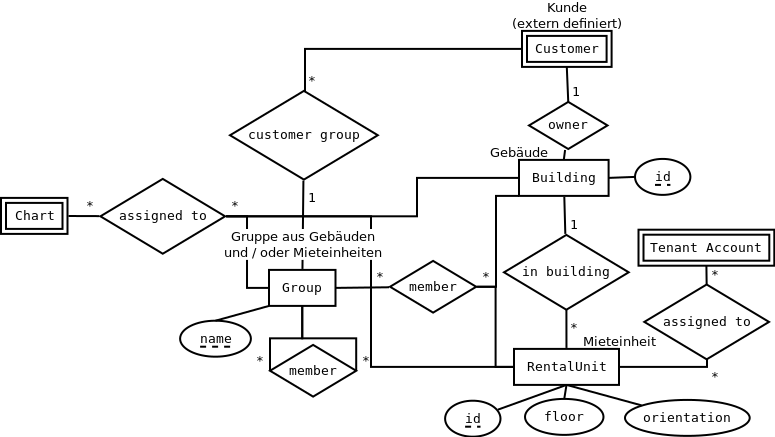
\includegraphics[width=130mm]{company_structure.png}
		\caption{Firmenstruktur der Kunde}
	\end{figure}
	\begin{figure}[h]
		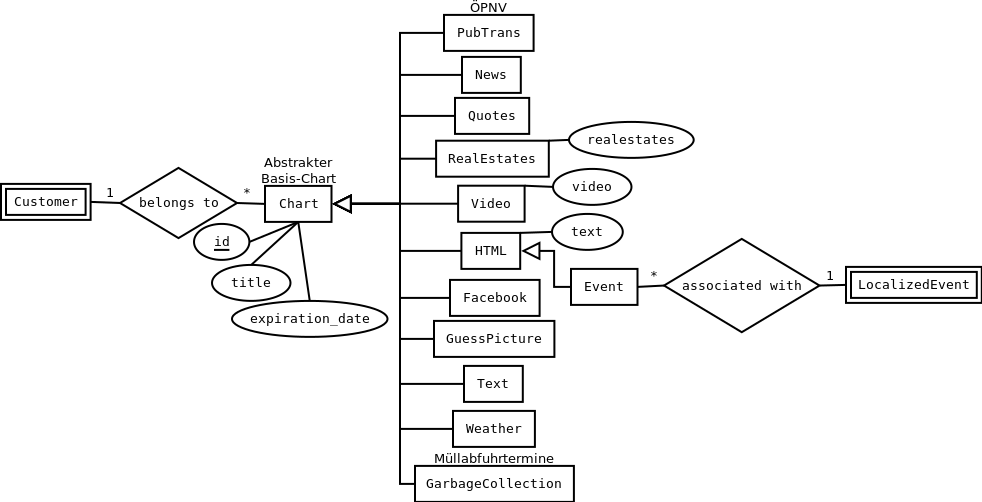
\includegraphics[width=130mm]{charts.png}
		\caption{Charts}
	\end{figure}
	\begin{figure}[h]
		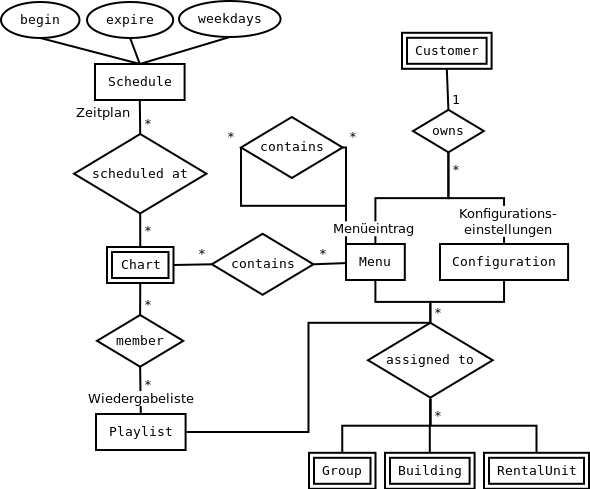
\includegraphics[width=100mm]{presentation.png}
		\caption{Präsentationsdaten}
	\end{figure}
	\begin{figure}[h]
		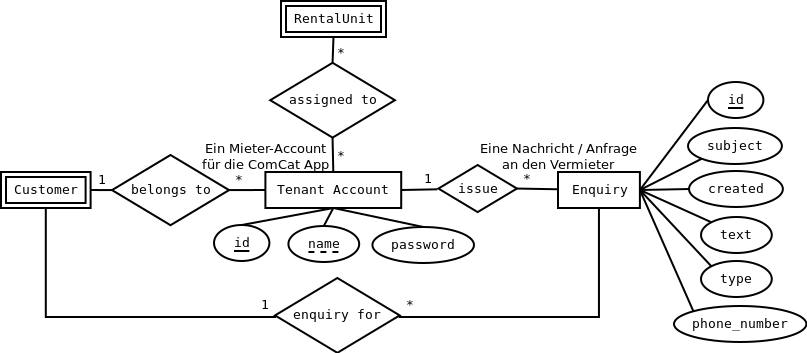
\includegraphics[width=130mm]{comcat.png}
		\caption{ComCat}
	\end{figure}
	\begin{figure}[h]
		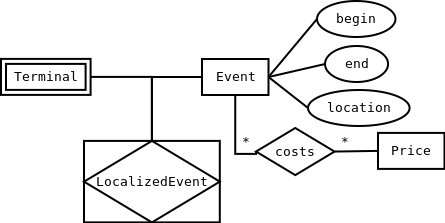
\includegraphics[width=130mm]{static_data.png}
		\caption{Statische Zusatzdaten}
	\end{figure}
	\end{center}
	\FloatBarrier
	\subsection{ReST API}
	Das zentrale ReST API soll die \emph{Datenverarbeitung} des Systems übernehmen und als \emph{zentraler Server} von \enquote{ComCat} fungieren.
	Daraus ergeben sich folgende funktionale Anforderungen:
	\begin{itemize}
		\item	Bereitstellung einer standardkonformen ReST Schnittstelle über HTTPS
		\item Authentifizierung von Benutzern
		\item Autorisierung von Benutzern
		\item Verwaltung von Mietobjekten
		\item Verwaltung von Dienstleistern
		\item Verwaltung von Inhalten
		\item Verwaltung von Meldungen
		\item Zuordnung von Inhalten zu Mietobjekten
		\item Zuordnung von Meldungen zu Dienstleistern
	\end{itemize}
	\subsection{Smartphone App für Mieter}
	Die Smartphone App soll als Client des ReST API fungieren.
	\begin{itemize}
		\item Abfrage von Inhalten zum Mietobjekt
		\item Versand von Meldungen an den Vermieter
	\end{itemize}
	\subsection{Content Management System}
	Das CMS soll auf allen gängigen Webbrowsern lauffähig sein.
	\subsection{Use-Case-Diagramme}
	\subsection{Use-Case Tabellen}
	\subsubsection{Smartphone App}
	\paragraph{Mieter App}
	\begin{tabular}{|l|p{9cm}|}
		\hline
		\emph{Use Case Nr. 1} & Login \\
		\hline
		\emph{Umfeld} & Smartphone \\
		\hline
		\emph{Systemgrenzen} & ReST API \\
		\hline
		\emph{Ebene} & App \\
		\hline
		\emph{Hauptakteur} & Smartphone Benutzer \\
		\hline
		\emph{Stakeholder u. Interesse} & Mieter möchte sich in der \emph{Smartphone App} anmelden \\
		\hline
		\emph{Voraussetzung} & Aktive Netzwerkverbindung, App gestartet \\
		\hline
		\emph{Garantien} & – \\
		\hline
		\emph{Erfolgsfall} & Anmeldung erfolgreich und Anzeige aktueller Meldungen zum Wohnobjekt \\
		\hline
		\emph{Auslöser} & Betätigen der Schaltfläche \enquote{Anmelden} \\
		\hline
		\emph{Beschreibung} & 
			\begin{tabular}{lp{8cm}}
				1. & Eintippen den korrekten Chiffre im dafür vogesehenen Textfeld \\
				2. & Betätigen der Schaltfläche \enquote{Anmelden}  \\
			\end{tabular}  
		WEITER: Use Case 2 \\
		\hline
		\emph{Erweiterungen} & 
		\begin{tabular}{lp{8cm}}
			2a & WENN die Anmeldung fehlschlägt,  DANN Warnmeldung anzeigen \\
		\end{tabular} \\
		\hline
		\emph{Technologie} & HTTPS \\
		\hline

	\end{tabular}
	
	\pagebreak
	
	\section{Skizzen}
	Im Folgenden werden Skizzen zur grafischen Benutzeroberfläche der \emph{Smartphone App} gezeigt, die als Vorlage für die spätere Implementierung dienen sollen.
	\begin{figure}[H]
		\centering
	%	\includegraphics[width=0.7\linewidth]{./GUI/PET-Login}
		\caption{Smartphone App Mockup}
		\label{fig1}
	\end{figure}
	\subsection{Programmabläufe}
	keine
	
	\section{Glossar}
	% Glossar ausgeben
	\printglossaries

\end{document}
